\documentclass[12pt]{article}
% Préambule commun à tous les documents extraits de « La Revue CAPES »
\usepackage[T1]{fontenc}
\usepackage[utf8]{inputenc}
\usepackage{lmodern}
\usepackage{amsmath,amssymb,amsthm,amsfonts,mathrsfs}
\usepackage{setspace}
\usepackage{listings}
\usepackage{pgfplots}
\pgfplotsset{compat=1.18}
\usepackage{longtable}
\usepackage{adjustbox}
\usepackage{lettrine}
\usepackage{tkz-tab}
\usepackage{changepage}
\usepackage{pdflscape}
\usepackage{graphicx}
\usepackage{tikz}
\usepackage{xcolor}
\usepackage[a4paper,top=2cm,bottom=2.5cm,left=2.5cm,right=2cm]{geometry}
\usepackage{fancyhdr}
\usepackage{draftwatermark}
\SetWatermarkText{La RevueCapes}
\SetWatermarkLightness{0.9}
\SetWatermarkScale{2}
\usepackage{hyperref}
\hypersetup{colorlinks=true,linkcolor=blue!50!black,urlcolor=blue!50!black}

\definecolor{revue}{RGB}{20,60,120}

\pagestyle{fancy}
\fancyhf{}
\renewcommand{\headrulewidth}{0.4pt}
\setlength{\headheight}{15pt}

% \entete{Matière}{Titre}{Type de document}
\newcommand{\entete}[3]{%
  \fancyhead[L]{\small\textsc{La Revue CAPES} -- #1}%
  \fancyhead[R]{\small #2}%
  \fancyfoot[C]{\thepage}%
  \thispagestyle{plain}%
  \begin{center}
    {\color{revue}\rule{\textwidth}{1.2pt}}\\[4pt]
    {\small\textsc{Concours directs CAP-CEG / CAPES -- Burkina Faso}}\\[6pt]
    {\LARGE\bfseries\color{revue} #2}\\[6pt]
    {\large\itshape #1 -- #3}\\[2pt]
    {\color{revue}\rule{\textwidth}{1.2pt}}
  \end{center}
  \vspace{0.5cm}%
}

% Encadré pour les remarques ajoutées dans les corrigés
\newcommand{\remarque}[1]{\par\medskip\noindent\fcolorbox{revue}{revue!6}{\parbox{\dimexpr\linewidth-2\fboxsep-2\fboxrule}{\textbf{\color{revue}Remarque.} #1}}\par\medskip}


\begin{document}
\entete{Mathématiques}{Corrigé détaillé du sujet type n°7}{Correction}
\begin{spacing}{1.5}

\textbf{Exercice 1}






\medskip
1. Déterminons l'ensemble des valeurs possibles pour \(x\) et \(y\)

On a :
\[
x(t) = \frac{t^2}{t^2 + 1}, \quad y(t) = \frac{t^3}{t^2 + 1}.
\]

\textbf{Pour \(x\) :}
\[
x(t) = \frac{t^2}{t^2 + 1}.
\]
\begin{itemize}
    \item \(t^2 \geq 0 \implies x(t) \geq 0\),
    \item lorsque \(t \to 0\), \(x(t) \to 0\),
    \item lorsque \(t \to \pm\infty\), \(x(t) \to \frac{t^2}{t^2} = 1\).
\end{itemize}

Ainsi, \(x(t) \in [0, 1[\).

\textbf{Pour \(y\) :}
\[
y(t) = \frac{t^3}{t^2 + 1}.
\]
\begin{itemize}
    \item Lorsque \(t = 0\), \(y(0) = 0\),
    \item Lorsque \(t > 0\), \(t^3 > 0\), donc \(y(t) > 0\),
    \item Lorsque \(t < 0\), \(t^3 < 0\), donc \(y(t) < 0\),
    \item Lorsque \(t \to \pm\infty\), \(y(t) \to \frac{t^3}{t^2} = t\).
\end{itemize}

Ainsi, \(y(t)\) prend toutes les valeurs dans \(\mathbb{R}\).

\medskip
2. Montrons que \(O(0,0)\) appartient à \(C\)

Pour \(t = 0\), on calcule :
\[
x(0) = \frac{0^2}{0^2 + 1} = 0, \quad y(0) = \frac{0^3}{0^2 + 1} = 0.
\]

Le point \(O(0,0)\) appartient donc à la courbe \(C\).

\textbf{Pente de la tangente au point \(O\) :}

La pente de la tangente est donnée par :
\[
p = \frac{\mathrm{d}y}{\mathrm{d}x}.
\]

On calcule les dérivées paramétriques de \(x(t)\) et \(y(t)\) :
\[
x'(t) = \frac{2t(t^2 + 1) - t^2 \cdot 2t}{(t^2 + 1)^2} = \frac{2t}{(t^2 + 1)^2},
\]
\[
y'(t) = \frac{3t^2(t^2 + 1) - t^3 \cdot 2t}{(t^2 + 1)^2} = \frac{t^2(3 - t^2)}{(t^2 + 1)^2}.
\]

Ainsi :
\[
\frac{\mathrm{d}y}{\mathrm{d}x} = \frac{y'(t)}{x'(t)} = \frac{\frac{t^2(3 - t^2)}{(t^2 + 1)^2}}{\frac{2t}{(t^2 + 1)^2}} = \frac{t(3 - t^2)}{2}.
\]

Au point \(O\) (\(t = 0\)) :
\[
p = \frac{0(3 - 0^2)}{2} = 0.
\]

La tangente à la courbe au point \(O\) est donc horizontale.

\medskip
3. Équation de la courbe \(C\) sous forme \(y = g(x)\)

On exprime \(t\) en fonction de \(x\) à partir de \(x(t) = \frac{t^2}{t^2 + 1}\) :
\[
x = \frac{t^2}{t^2 + 1} \implies t^2 = \frac{x}{1 - x} \quad (\text{pour } x \in [0, 1[).
\]

En prenant \(t = \pm\sqrt{\frac{x}{1 - x}}\), on substitue dans \(y(t)\) :
\[
y = \frac{t^3}{t^2 + 1} = \frac{\left(\pm\sqrt{\frac{x}{1 - x}}\right)^3}{\frac{x}{1 - x} + 1}.
\]

Cela donne :
\[
y = \pm\frac{\left(\frac{x}{1 - x}\right)^{3/2}}{\frac{1}{1 - x}} = \pm \sqrt{\frac{x^3}{1 - x}}.
\]

Ainsi, l'équation de \(C\) est donnée par :
\[
y = \pm\sqrt{\frac{x^3}{1 - x}}, \quad x \in [0, 1[.
\]

\textbf{Calcul de \(y'\) et variations de \(g(x)\) :}

Pour \(y = \sqrt{\frac{x^3}{1 - x}}\), on a :
\[
y' = \frac{1}{2\sqrt{\frac{x^3}{1 - x}}} \cdot \frac{(1 - x) \cdot 3x^2 + x^3}{(1 - x)^2} = \frac{(2 - x)x}{2(1 - x)\sqrt{\frac{x^3}{1 - x}}}.
\]

Les variations de \(g(x)\) dépendent du signe de \(y'\). En analysant, la courbe \(C\) est symétrique par rapport à l'origine et a une branche croissante pour \(x \in [0, 1[\).

La courbe \(C\) a donc une forme générale qui ressemble à une boucle.





\quad


\begin{center}
\textbf{Courbe \(C\) : \(y = \pm \sqrt{\frac{x^3}{1-x}}\)}


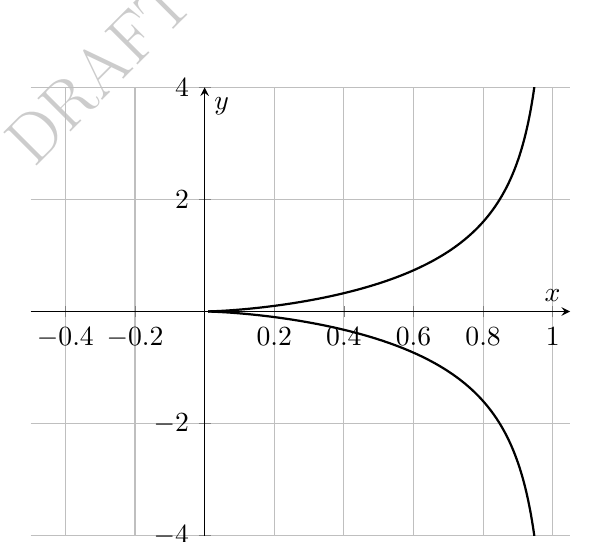
\begin{tikzpicture}
    \begin{axis}[
        axis lines = middle,
        xlabel = $x$,
        ylabel = $y$,
        ymin = -4, ymax = 4,
        xmin = -0.5, xmax = 1.05,
        domain = 0.01:0.99, % Évite les singularités aux limites
        samples = 600,
        legend pos = north west,
        grid = both
    ]
        % Courbe positive
        \addplot[
            color=black,
            thick
        ]{sqrt(x^3/(1-x))};
  %      \addlegendentry{$y = +\sqrt{\frac{x^3}{1-x}}$}
        
        % Courbe négative
        \addplot[
            color=black,
            thick
        ]{-sqrt(x^3/(1-x))};
      %  \addlegendentry{$y = -\sqrt{\frac{x^3}{1-x}}$}
    \end{axis}
\end{tikzpicture}
\end{center}




\quad

\medskip\textbf{Exercice 2} 

Soit $f$ la fonction définie sur $\mathbb{R}_{+}^{*}$ par
 \[
 \begin{cases}
 f(0)=0\\
 f(x)= \frac{x^2}{sh x}
 \end{cases}
 \]
 
 1. Déterminons le développement limité d'ordre 5 de $e^x$ et de $sh x$ en 0.
 
 \[e^x=\sum_{k=0}^n\frac{x^k}{k!}=1+x+\frac{1}{2}x^2+\frac{1}{6}x^3+\frac{1}{24}x^4+\frac{1}{120}x^5 + \circ(x^5)\]
 
 
\[sh x=\sum_{k=0}\frac{x^{2k+1}}{(2k+1)!}=x+\frac{x^3}{6}+\frac{x^5}{120}+\circ(x^5)\] 
 
 2. Déduisons le développement limité d'ordre 3 de $f$ en 0.
 
 \[f(x)=\frac{x^2}{sh x}=\frac{x^2}{x+\frac{x^3}{6}+\frac{x^5}{120}+\circ(x^5)}=\frac{x}{1+\frac{x^2}{6}+\frac{x^4}{120}+\circ(x^4)}=x-\frac{x^3}{6}+\circ(x^3)\](Obtenue par division euclidienne)
 
 3. Déduisons que $f$ est dérivable sur $\mathbb{R}$ et précisons la position relative au voisinage de 0 du graphe de $f$ par rapport à sa tangente en 0.
 
 $f(x)=x-\frac{x^3}{6}+\circ(x^3)$ est un polynôme donc dérivable sur $\mathbb{R}$
 
 Sa tangente en 0 est donnée par $(T): y=x$.
 
 On a : $f(x)-x=-\frac{x^3}{6}+\circ(x^3)\leq 0\forall x\in \mathbb{R}_{+}^{*}$ alors $(C_f)$ est en dessous de $(T)$.
 
 
 4. Déduisons $f^{(3)}(0)$.
 
 \[f'(0)=1 \text{  } , f''(0)= 0 \text{  }, f^{(3)}(0)=-\frac{1}{6}\]
 
 En effet, 
 
 \[f(x)=f(0)+xf'(0)+x^2f''(0)+x^3f^{(3)}(0)=x-\frac{x^3}{6}\]
 
 Par identification, on trouve les résultats ci-dessus.
 

\medskip\textbf{Exercice 3}


1.(a) Le nombre de codes possible :

Chaque chiffre peut être compris entre 1 et 9.

Nombre total de combinaisons : $9\times 9\times 9 =$\textbf{ 729 codes.}

(b) Nombre de codes se terminant par un chiffre impair :

Les chiffres impairs sont : 1,3,5,7,9 (5 possibilités).

Les deux premiers chiffres du code peuvent être quelconque : $9\times 9$.

Ainsi le nombre de codes se terminant par un chiffre impair est : $9\times 9\times 5=405$ codes.

\medskip
Déduisons le nombre de codes se terminant par un chiffres pair :

Par différence, le nombre de codes se terminant par un chiffre pair est :  729-405=\textbf{ 324 codes}.

(c) Nombre de codes contenant au plus un chiffre 5 :

On dénombre ici ou il n'y a aucun chiffre 5 ou il y a exactement un chiffre 5.

$\bullet$ \textbf{Aucun chiffre 5 :} chaque chiffre peut être 1,2,3,4,6,7,8,9 (8 possibilités).

Nombre de codes dans ce cas : $8\times 8\times 8=512$  codes

$\bullet$ \textbf{Exactement un chiffre 5 :} 5 peut être placé à l'une des 3 positions( choix des positions $C_3^1=3$). Les deux autres chiffres sont choisis parmi 1,2,3,4,6,7,8,9 ( 8 possibilités chacun)

Nombre de codes : $3\times 8\times 8 = 192$ codes.

$\quad$

Ainsi le nombre total de codes avec au plus un chiffre 5 est :512+192 codes = \textbf{704 codes}


(d) Le nombre de codes ne contenant pas le chiffre 5.

Tous les chiffres sont choisis parmi 1,2,3,4,6,7,8,9(8 possibilités).

Nombre de codes : $8\times 8\times 8$= \textbf{512 codes}.

\quad

2.(a) Nombre de codes possibles

Les chiffres doivent être distincts :

$\bullet$ \underline{$1^{er}$ chiffre :} 9 choix.

$\bullet$ \underline{$2^{eme}$ chiffre :} 8 choix (différent du premier).

$\bullet$ \underline{$3^{eme}$ chiffre :} 7 choix (différent des deux premiers).

Nombre total des combinaisons possibles : $9\times 8\times 7$= \textbf{504 codes}

(b) Le nombre de codes se terminant par un chiffre pair :

Le dernier chiffre est choisi parmi les chiffres pairs (2,4,6,8) (4 possibilités).

Les deux premiers chiffres sont choisis parmi les 8 chiffres restants de façon distincts : 8 choix pour le premier et 7 choix pour le deuxième.

Nombre de codes : $8\times 7\times 4$=\textbf{224 codes}

\quad

Déduisons le nombre de codes se terminant par un chiffre impair :


Par différence, le nombre de codes se terminant par un chiffre impair est : 504-224 = \textbf{280 codes}


(c) Nombre de codes comprenant les chiffres 5 et 7 :

$\cdot$ Les chiffres 5 et 7 doivent être dans le code.

$\cdot$ Choix des positions des chiffres 5 et 7 dans les trois places : $C_3^2=3$

$\cdot$ Le troisième chiffre est choisi parmi les 7 chiffres restants (distincts de 5 et 7).

Nombre de codes : $3\times 7=$\textbf{ 21 codes}


\quad

\textbf{Exercice 4}

La fonction f est définie sur $\mathbb{R}^2$ par :
\[
f(x, y) = 2x^3 + xy^2 + 5x^2 + y^2.
\]

1. Recherche d'un maximum ou minimum global

Pour déterminer si $f$ possède un maximum ou minimum global sur $\mathbb{R}^2$, nous analysons le comportement de $f(x, y)$ lorsque $\|(x, y)\| \to \infty$.

\[
f(x, y) = 2x^3 + xy^2 + 5x^2 + y^2.
\]

Lorsque $x \to \pm \infty$, le terme dominant est $2x^3$, qui diverge respectivement vers $+\infty$ ou $-\infty$. Donc, $f(x, y)$ ne possède pas de borne supérieure ni de borne inférieure. 

Conclusion : La fonction $f$ n'a pas de maximum ni de minimum global sur $\mathbb{R}^2$.

2. Recherche des extrémums locaux

Pour trouver les points où $f$ présente des extrémums locaux, calculons le gradient de $f$ :
\[
\nabla f(x, y) = \left( \frac{\partial f}{\partial x}, \frac{\partial f}{\partial y} \right).
\]

Les dérivées partielles sont :
\[
\frac{\partial f}{\partial x} = 6x^2 + y^2 + 10x, \quad \frac{\partial f}{\partial y} = 2xy + 2y.
\]

Pour trouver les points critiques, résolvons le système :
\[
\frac{\partial f}{\partial x} = 0 \quad \text{et} \quad \frac{\partial f}{\partial y} = 0.
\]

\textbf{ Résolution du système}

 $\frac{\partial f}{\partial y} = 2y(x + 1) = 0$ \\
   Cette équation donne deux cas :
\[
   y = 0 \quad \text{ou} \quad x = -1.
\]

 Étudions chaque cas :

   - Si $y = 0$, alors $\frac{\partial f}{\partial x} = 6x^2 + 10x = 0$, soit :
\[
     x(6x + 10) = 0 \implies x = 0 \quad \text{ou} \quad x = -\frac{5}{3}.
\]

   - Si $x = -1$, alors $\frac{\partial f}{\partial x} = 6(-1)^2 + y^2 + 10(-1) = y^2 - 4 = 0$, soit :
\[
     y^2 = 4 \implies y = \pm 2.
\]

$\cdot$ \textbf{Points critiques}

Les points critiques de $f$ sont donc :
\[
(0, 0), \quad \left(-\frac{5}{3}, 0\right), \quad (-1, 2), \quad (-1, -2).
\]

$\cdot$ \textbf{ Nature des points critiques}

Pour déterminer la nature des points critiques (minimum local, maximum local ou point selle), calculons la matrice hessienne de $f$ :
\[
H_f(x, y) = 
\begin{pmatrix}
\frac{\partial^2 f}{\partial x^2} & \frac{\partial^2 f}{\partial x \partial y} \\
\frac{\partial^2 f}{\partial y \partial x} & \frac{\partial^2 f}{\partial y^2}
\end{pmatrix}.
\]

Les dérivées secondes sont :
\[
\frac{\partial^2 f}{\partial x^2} = 12x + 10, \quad 
\frac{\partial^2 f}{\partial y^2} = 2x + 2, \quad 
\frac{\partial^2 f}{\partial x \partial y} = \frac{\partial^2 f}{\partial y \partial x} = 2y.
\]

La matrice hessienne est donc :
\[
H_f(x, y) = 
\begin{pmatrix}
12x + 10 & 2y \\
2y & 2x + 2
\end{pmatrix}.
\]

$\cdot$ Étudions la nature des points critiques :

- Point $(0, 0)$ :
\[
   H_f(0, 0) = 
   \begin{pmatrix}
   10 & 0 \\
   0 & 2
   \end{pmatrix}.
\]

   Les valeurs propres sont $10 > 0$ et $2 > 0$. Donc, $(0, 0)$ est un \textbf{minimum local}.

- Point $\left(-\frac{5}{3}, 0\right)$ :
\[
   H_f\left(-\frac{5}{3}, 0\right) = 
   \begin{pmatrix}
   12\left(-\frac{5}{3}\right) + 10 & 0 \\
   0 & 2\left(-\frac{5}{3}\right) + 2
   \end{pmatrix} = 
   \begin{pmatrix}
   0 & 0 \\
   0 & -\frac{4}{3}
   \end{pmatrix}.
\]

   La matrice n'est pas définie, donc $\left(-\frac{5}{3}, 0\right)$ est un \textbf{point selle}.

- Point $(-1, 2)$ :
\[
   H_f(-1, 2) = 
   \begin{pmatrix}
   12(-1) + 10 & 4 \\
   4 & 2(-1) + 2
   \end{pmatrix} = 
   \begin{pmatrix}
   -2 & 4 \\
   4 & 0
   \end{pmatrix}.
\]

   Le déterminant est $\det(H_f(-1, 2)) = (-2)(0) - (4)(4) = -16 < 0$. Donc, $(-1, 2)$ est un \textbf{point selle}.

- Point $(-1, -2)$ :*
\[
   H_f(-1, -2) = 
   \begin{pmatrix}
   -2 & -4 \\
   -4 & 0
   \end{pmatrix}.
\]

   Le déterminant est $\det(H_f(-1, -2)) = -16 < 0$. Donc, $(-1, -2)$ est un \textbf{point selle}.
   
   \medskip

\textbf{ Conclusion}

- $(0, 0)$ est un \textbf{minimum local}.
- $\left(-\frac{5}{3}, 0\right), (-1, 2), (-1, -2)$ sont des \textbf{points selle}.

\end{spacing}
\end{document}
